\section{Other commonly DWS-Architectures}
\label{sec:otherArchitectures}

\subsection{Distributed Data Warehousing Architecture}
After having explained the reference architecture from A. Bauer which implements the hub and spoke idea from Inmon one very common alternative is presented. Ralph Kimball is another pioneer in this area who came up with a distributed data warehousing architecture based upon data marts connected to a bus system. \cite{surveyDWSArchs} Figure \ref{fig:distributedWarehouseArchitecture} visualises this in more detail.
\begin{figure}[htb]
    \centering
    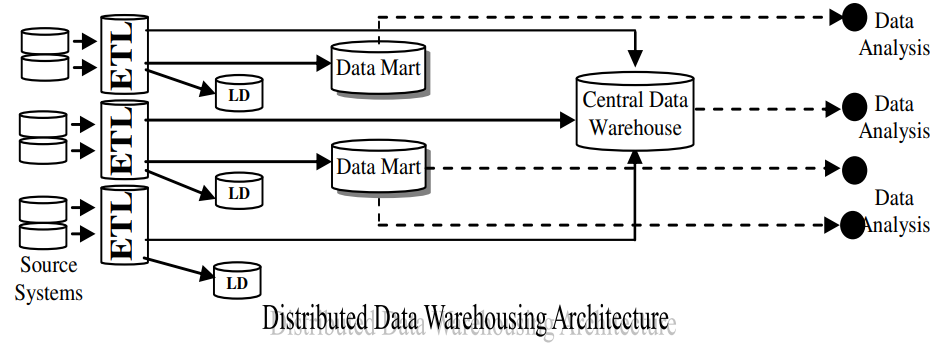
\includegraphics[scale=0.5]{pictures/DistributedDataWarehouseArchitecture.PNG}
    \caption{Distributed Data Warehousing Architecture by Ralph Kimball \cite{surveyDWSArchs}}
    \label{fig:distributedWarehouseArchitecture}
\end{figure}
\\In contrast to Inmon's approach Kimball allows 'Everyone [...] to fabricate their database according to their requirements and department structures. All there independent repositories can be integrated as and when. [...]' \cite{surveyDWSArchs}. Due to that the Central / Core Data Warehouse results from those individual Data Mart and doesn't provide any consistency. This technique is also known as bottom-up approach for developing Data Warehouse Systems. Since the bus system is needed to ensure the interoperability between multiple data marts and the core data warehouse consistent data standards are therefore needed. Due to that the design aspects are quite tough and the complexity is high. \cite{KimbalVSInmon}\newline
As Breslin states 'Kimball's approach is a departure from traditional database development'\cite[p.~19]{KimbalVSInmon} and therefore targets the IT-Professional himself.\newline
\\
After the most commonly used architectures for Data Warehouse Systems have been outlined and the requirements regarding a DWS are pointed out, some newer technologies are introduced. In detail the fundamental ideas of micro-service and event-based architectures as well as Business Process Management will be elaborated. Further on these technologies will align in order to result into the final draft of the presented architecture.

\subsection{Architectural Classification according to the Arrangement of Data Marts}

